%!TEX root = main.tex

\textbf{Problem}: Machine translation concenrs the use of computers to automate translation from a source language to a target language.

\subsubsection{Why is MT difficult ?}

\begin{itemize}
	\item \textbf{Strucutral divergences};
	\begin{itemize}
		\item \textbf{Isolating} (one morphene per word) vs \textbf{polysynthetic} (one word is a sentence);
		\item \textbf{Word orders};
		\item \textbf{Argument structure}: verb-framed, satellite-framed;
		\item \textbf{Pronoun dropping};
		\item \textbf{Specific divergences}: adjective precede or not nouns.
	\end{itemize}
	\item \textbf{Lexical divergences}.
	\begin{itemize}
		\item \textbf{Homonymous words}: ex. \textit{bass};
		\item \textbf{Polysemous words}: ex. \textit{know};
		\item \textbf{Grammatical lexical divergences}: ex. gender on adjectives;
		\item \textbf{Lexical gaps}: no word in one language.
	\end{itemize}
\end{itemize}

\subsubsection{Various translation tasks}

\begin{itemize}
	\item \textbf{Rough translation};
	\item \textbf{Draft translation with human post-editing};
	\item \textbf{Fully automatic translation}.
\end{itemize}

\subsection{Approaches}

\begin{figure}[htp]
	\centering
	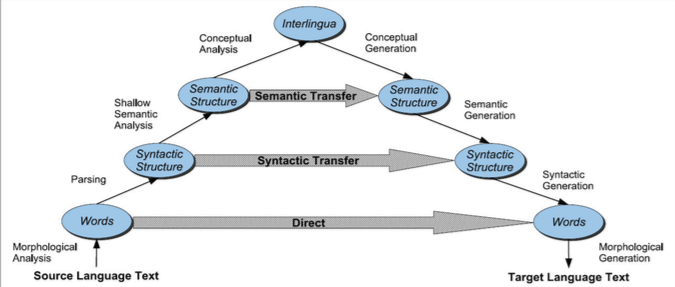
\includegraphics[scale=0.6]{images/58_levels.png}
 	\caption{Levels of transfer.}
\end{figure}

\subsubsection{Direct transfer}

Word-by-word through the source language text, incrementally transforming the source language text into a target language text (bilingual dictionary for lexical transfer).

\paragraph{Limitations}
\begin{itemize}
	\item Complex and numerous transformation rules;
	\item No parsing component (cannot handle reliably long distance reordering).
\end{itemize}

\subsubsection{Syntactic and semantic transfer}

Parse, then transfer the syntactic structure and finally generate the target text.

\paragraph{Limitations}
\begin{itemize}
	\item Translating from SVO languages to SOV languages require complex syntactic transformations;
	\item Lexical transfer is also required with a bilingual dictionary but unsatisfactory for ambiguous words;
	\item Additional semantic analysis is required but it is even more complex to define reliable semantic transformations.
\end{itemize}

\subsubsection{Interlingua}

Treat translation as a process of extracting the full meaning of the source and expressing it in the target language.

\paragraph{Limitations}
\begin{itemize}
	\item Deep conceptual analysis is even more difficult than shallow semantic analysis;
	\item The generation steps are far from trivial;
	\item Some concepts simply do not exist in common between languages.
\end{itemize}

\subsection{Statistical machine translation}

\begin{figure}[htp]
	\centering
	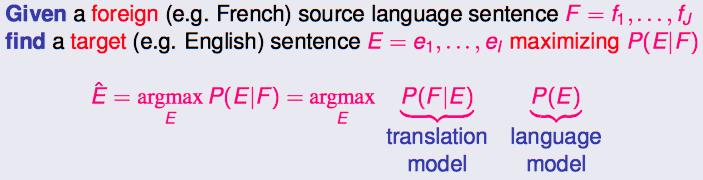
\includegraphics[scale=0.4]{images/59_def.png}
 	\caption{Problem definition. Require: a \textbf{language model} to compute P(E); a \textbf{translation model} to compte P(F|E); a \textbf{decoder} to compute $\hat{E} = \text{argmax}_E P(F|E) P(E)$.}
\end{figure}
\begin{figure}[htp]
	\centering
	
\includegraphics[scale=0.5]{images/60_best.png}
 	\caption{Best translation. Trade-off.}
\end{figure}

\begin{figure}[H]
	\centering
	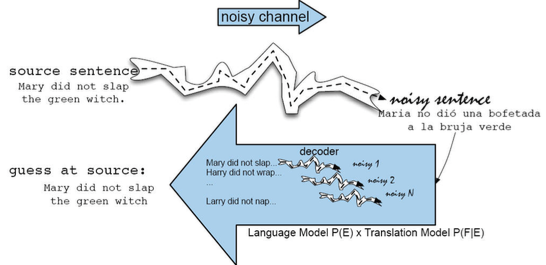
\includegraphics[scale=0.6]{images/61_noisy.png}
 	\caption{The speaker think in English and produce a  noisy version in aother language. The translation aims at decoding the noisy version.}
\end{figure}


\begin{figure}[H]
	\centering
	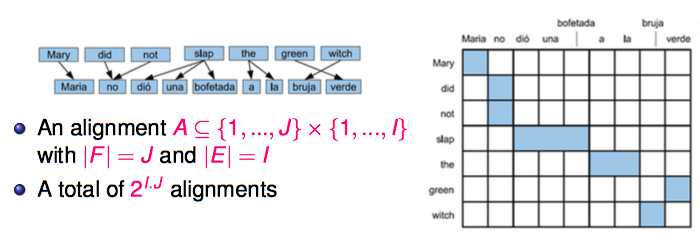
\includegraphics[scale=0.6]{images/62_ali.png}
 	\caption{Alignments.}
\end{figure}

\subsubsection{Phrase-based models}

Phrases are units of translation, each phrase has exactly one translation, then alignments are permutations. The model includes \textbf{translation probabilities} of phrases and \textbf{distortion probabilities} to model the permutations.

\begin{figure}[H]
	\centering
	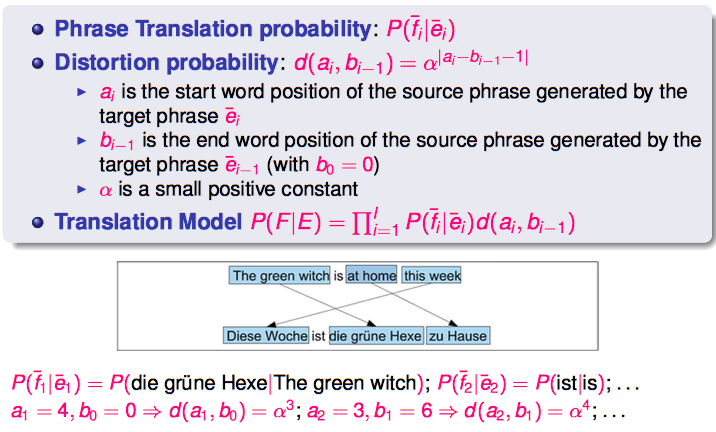
\includegraphics[scale=0.6]{images/63_phrase.png}
 	\caption{Phrase-based translation model. Parameters are $P(\bar{f}|\bar{e})$ and $\alpha$.}
\end{figure}

A such model is essentially a large bilingual probabilistic dictionary of phrases which can be estimated from a large corpus of aligned phrases and their respective counts C(.,.), but aligned phrases are rarely available as such in parallel corpora and then word alignments are used as seeds for phrase alignments.

\begin{figure}[H]
	\centering
	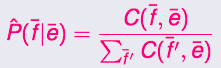
\includegraphics[scale=0.6]{images/64_param.png}
 	\caption{Large bilingual probabilistic dictionary.}
\end{figure}


\begin{figure}[H]
	\centering
	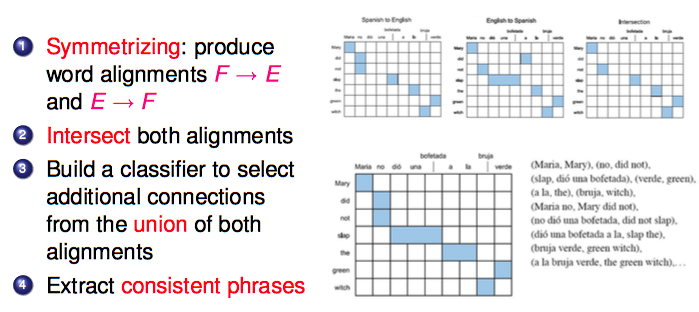
\includegraphics[scale=0.6]{images/65_ali.png}
 	\caption{Words to phrase alignments algorithm.}
\end{figure}

\subsubsection{Multi-stack decoding with phrase-based models}

\begin{figure}[htp]
	\centering
	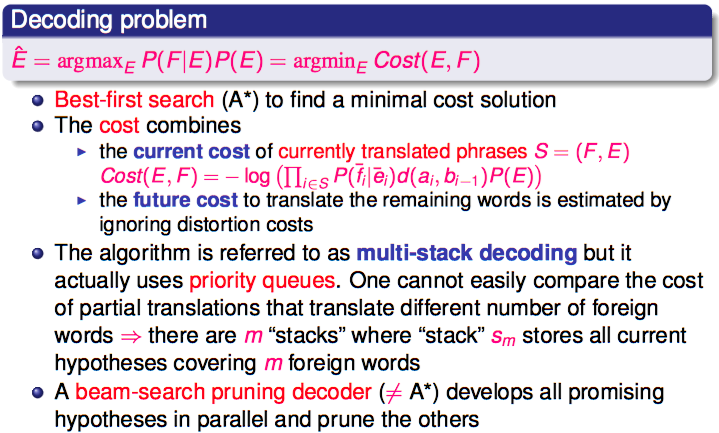
\includegraphics[scale=0.6]{images/66_stacks.png}
 	\caption{Multi-stack decoding with phrase-based models.}
\end{figure}

\subsection{MT evaluation}

\subsubsection{Criteria}

\begin{itemize}
	\item \textbf{Human raters}:
	\begin{itemize}
		\item \textbf{Fluency}: clarity, naturalness;
		\item \textbf{Faithfulness}: adequacy;
		\item \textbf{Informativeness}: enough information to accomplish a task;
		\item \textbf{Edit-cost}: minimizing post editing.
	\end{itemize}
	\item \textbf{Automatic evaluation}:
	\begin{itemize}
		\item Heuristics to assess translation systems automatically with respect to reference translations provided by humans;
		\item Correlated with human judgments.
	\end{itemize}
\end{itemize}

\subsubsection{BLEU evaluation metric}

\begin{figure}[htp]
	\centering
	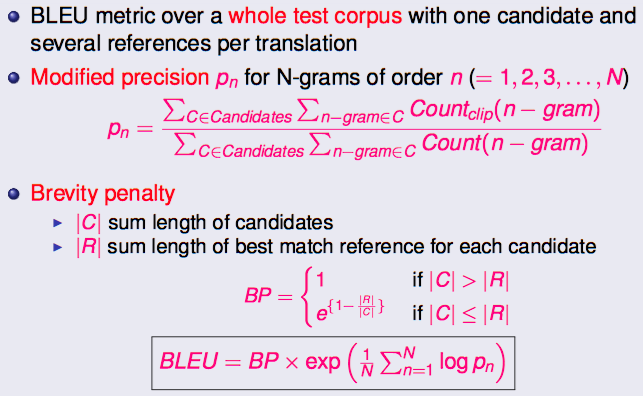
\includegraphics[scale=0.6]{images/67_bleu.png}
 	\caption{BLEU.}
\end{figure}
